\documentclass{ajhlabreport}
\usepackage{ajhdsp}

\newcommand{\generatedfigw}[2]{
	\includegraphics[width=#1\textwidth]{generated/#2.png}
}

\setlength{\parindent}{0bp}

\datedue{November 15, 2012\footnote{postponed to November 29, 2012 due to academic schedule}}
\class{EE4252}
\submittedto{\href{mailto:yliu18@mtu.edu}{Yang Liu}}
\pretitle{Lab 8 Report}
\title{Analog Filters}
\author{\href{mailto:ahirzel@mtu.edu}{Alex Hirzel}}

\begin{document}
\maketitle




\chapter{Project 1: Basic Analog Filter Design}%%%%%%%%%%%%%%%%%%%%%%%%%%%%%%%%%

This project creates and compares four implementations of a band-pass filter.
Butterworth, Chebyshev I/II and elliptic design techniques are compared. All
designs are completed using \texttt{afdgui} and by hand.


\subsection{Butterworth filter}%%%%%%%%%%%%%%%%%%%%%%%%%%%%%%%%%%%%%%%%%%%%%%%%%

\begin{enumerate}[(a)]
%
\item This filter was designed using \texttt{afdgui} with band edges of $[ f_1,
f_2, f_3, f_4 ] = [ 10000, 16000, 25000, 50000 ]$ and attenuation specifications
$[ A_p, A_s ] = [ 1, 45 ]$. A screenshot of \texttt{afdgui} is shown below.
\begin{figure}[H]\centering\generatedfigw{0.8}{p1a-bw}\end{figure}
%
\item As seen in \autoref{lst:diary-txt}, the orders of the numerator and
denominator of the final band-pass filter are $5$ and $10$, respectively.
%
\item The low-pass prototype should be designed with order $5$ (because $2 \cdot
5$ poles will appear in the resulting denominator after transforming the LPP to
a band-pass.)
%TODO use formula
%
\item As seen in \autoref{lst:diary-txt}, the orders of the numerator and
denominator of the low-pass prototype are $0$ and $5$, respectively. The final
band-pass filter is this low-pass prototype transformed by a function involving
$s^2$, so the order of the final band-pass filter is expected to be $10$.
%
\item The pole-zero plot is shown in \autoref{fig:p1-bw-lpp-pz}. The pole
locations for the low-pass prototype appear to lie equi-spaced on the left half
of a circle. (This is expected.) There are no zeroes in the prototype.
%
\setcounter{enumi}{6}
\item Yes, the transfer functions match as seen in \autoref{lst:diary-txt}.
%
\end{enumerate}


\newpage
\subsection{Chebyshev I filter}%%%%%%%%%%%%%%%%%%%%%%%%%%%%%%%%%%%%%%%%%%%%%%%%%

\begin{enumerate}[(a)]
%
\item This filter was designed using \texttt{afdgui} with band edges of $[ f_1,
f_2, f_3, f_4 ] = [ 10000, 16000, 25000, 50000 ]$ and attenuation specifications
$[ A_p, A_s ] = [ 1, 45 ]$. A screenshot of \texttt{afdgui} is shown below.
\begin{figure}[H]\centering\generatedfigw{0.8}{p1a-c1}\end{figure}
%
\item As seen in \autoref{lst:diary-txt}, the orders of the numerator and
denominator of the final band-pass filter are $4$ and $8$, respectively.
%
\item The low-pass prototype should be designed with order $4$ (because $2 \cdot
4$ poles will appear in the resulting denominator after transforming the LPP to
a band-pass.)
%TODO use formula
%
\item As seen in \autoref{lst:diary-txt}, the orders of the numerator and
denominator of the low-pass prototype are $0$ and $4$, respectively. The final
band-pass filter is this low-pass prototype transformed by a function involving
$s^2$, so the order of the final band-pass filter is expected to be $8$.
%
\item The pole-zero plot is shown in \autoref{fig:p1-c1-lpp-pz}. The pole
locations for the low-pass prototype appear to lie equi-spaced on the left half
of an ellipse. (This is expected.) There are no zeroes in the prototype.
%
\setcounter{enumi}{6}
\item Yes, the transfer functions match as seen in \autoref{lst:diary-txt}.
%
\end{enumerate}


\newpage
\subsection{Chebyshev II filter}%%%%%%%%%%%%%%%%%%%%%%%%%%%%%%%%%%%%%%%%%%%%%%%%

\begin{enumerate}[(a)]
%
\item This filter was designed using \texttt{afdgui} with band edges of $[ f_1,
f_2, f_3, f_4 ] = [ 10000, 16000, 25000, 50000 ]$ and attenuation specifications
$[ A_p, A_s ] = [ 1, 45 ]$. A screenshot of \texttt{afdgui} is shown below.
\begin{figure}[H]\centering\generatedfigw{0.8}{p1a-c2}\end{figure}
%
\item As seen in \autoref{lst:diary-txt}, the orders of the numerator and
denominator of the final band-pass filter are $4$ and $8$, respectively.
%
\item The low-pass prototype should be designed with order $4$ (because $2 \cdot
4$ poles will appear in the resulting denominator after transforming the LPP to
a band-pass.)
%TODO use formula
%
\item As seen in \autoref{lst:diary-txt}, the orders of the numerator and
denominator of the low-pass prototype are $0$ and $4$, respectively. The final
band-pass filter is this low-pass prototype transformed by a function involving
$s^2$, so the order of the final band-pass filter is expected to be $8$.
%
\item The pole-zero plot is shown in \autoref{fig:p1-c2-lpp-pz}. The pole
locations for the low-pass prototype appear to lie equi-spaced on the left half
of an ellipse. (This is expected.) The zeroes are all on the $j\omega$ axis.
%
\setcounter{enumi}{6}
\item Yes, the transfer functions match as seen in \autoref{lst:diary-txt}.
%
\end{enumerate}


\newpage
\subsection{Elliptic filter}%%%%%%%%%%%%%%%%%%%%%%%%%%%%%%%%%%%%%%%%%%%%%%%%%%%%

\begin{enumerate}[(a)]
%
\item This filter was designed using \texttt{afdgui} with band edges of $[ f_1,
f_2, f_3, f_4 ] = [ 10000, 16000, 25000, 50000 ]$ and attenuation specifications
$[ A_p, A_s ] = [ 1, 45 ]$. A screenshot of \texttt{afdgui} is shown below.
\begin{figure}[H]\centering\generatedfigw{0.8}{p1a-el}\end{figure}
%
\item As seen in \autoref{lst:diary-txt}, the orders of the numerator and
denominator of the final band-pass filter are $5$ and $6$, respectively.
%
\item The low-pass prototype should be designed with order $3$ (because $2 \cdot
3$ poles will appear in the resulting denominator after transforming the LPP to
a band-pass.)
%TODO use formula
%
\item As seen in \autoref{lst:diary-txt}, the orders of the numerator and
denominator of the low-pass prototype are $2$ and $3$, respectively. The final
band-pass filter is this low-pass prototype transformed by a function involving
$s^2$, so the order of the final band-pass filter is expected to be $6$.
%
\item The pole-zero plot is shown in \autoref{fig:p1-el-lpp-pz}. The pole
locations for the low-pass prototype appear to lie equi-spaced on the left half
of an ellipse. (This is expected.) The zeroes are all on the $j\omega$ axis.
%
\setcounter{enumi}{6}
\item Yes, the transfer functions match as seen in \autoref{lst:diary-txt}.
%
\end{enumerate}


\newpage
\subsection{Summary}%%%%%%%%%%%%%%%%%%%%%%%%%%%%%%%%%%%%%%%%%%%%%%%%%%%%%%%%%%%%

\begin{enumerate}[(a)]
\setcounter{enumi}{10}
\item The elliptic filter ends up with the smallest order for these specs (order
3). This is expected, because the elliptic filter has the largest compromise:
ripple in both the passband and stopband. The designer is able to exploit this
tolerance of ripple to reduce the filter order, whereas the monotonic
Butterworth filter has a higher order but the (sometimes) useful property that
there is no ripple.
\end{enumerate}

\begin{figure}[H]
\centering
\subbottom[Pole-zero plot of Butterworth LPP.\label{fig:p1-bw-lpp-pz}]{\generatedfigw{0.4}{p1a-bw-pz}}
\subbottom[Pole-zero plot of Chevyshev I LPP.\label{fig:p1-c1-lpp-pz}]{\generatedfigw{0.4}{p1a-c1-pz}}
\subbottom[Pole-zero plot of Chebyshev II LPP.\label{fig:p1-c2-lpp-pz}]{\generatedfigw{0.4}{p1a-c2-pz}}
\subbottom[Pole-zero plot of elliptic LPP.\label{fig:p1-el-lpp-pz}]{\generatedfigw{0.4}{p1a-el-pz}}
\end{figure}



\newpage
\chapter{Project 2: Subsonic Filters}

The filter to be designed for this project would have a Bode plot of the
following general form:
%
\usetikzlibrary{decorations.text}
\begin{figure}[H]\centering
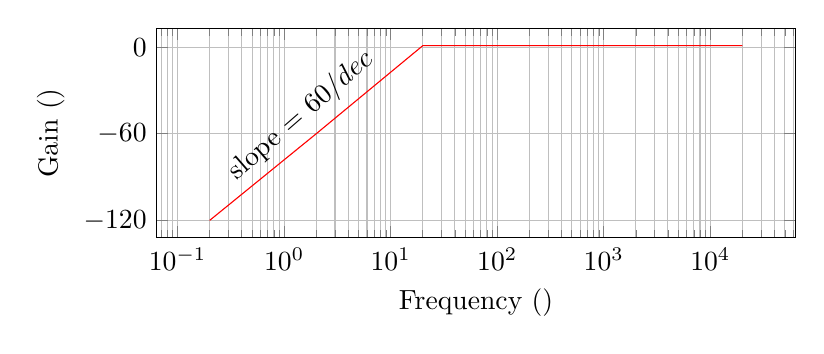
\begin{tikzpicture}
\begin{semilogxaxis}[
grid=both,
    height = 0.35\textwidth, width = 0.8\textwidth,
    ytick = {0,-60,-120},
    xlabel = {Frequency ($\hertz$)},
    ylabel = {Gain ($\deci\bel$}) ]
\addplot[color = red, no marks] coordinates { (0.2,-120) (2,-60) (20,1) (20000,1) };
\node[rotate = 41, above=0] at (axis cs: 2, -60) {slope = $60\deci\bel/\text{dec}$};
\end{semilogxaxis}
\end{tikzpicture}
\end{figure}
%
The Butterworth filter design will require the use of a third-order system
(because Butterworth filters inherently decay at $-20\deci\bel/\text{dec}$).
The functions \texttt{lpp} and \texttt{lp2af} were used to arrive at the final
filter design:
%
\begin{align*}
\boxed{H(s) = \frac{s^3}{s^3 + 251.1 s^2 + 31530 s + 1980000}}
\end{align*}
%
which has a frequency response as shown below:
%
\begin{figure}[H]\centering
\generatedfigw{0.9}{p2-final-bode}
\end{figure}



\newpage
\chapter{Project 3: A Multi-Band Filter}

\begin{enumerate}[(a)]
%
\item For Passband 1, a Butterworth filter must be used due to the ripple
requirements. A Chebyshev I filter can be used for Passband 2 because pass-band
ripples are permitted. The final filter was designed in MATLAB using
\texttt{afd} and has the following magnitude spectrum:
%
\begin{figure}[H]\centering
\generatedfigw{0.9}{p3-bode}
\end{figure}
%
\item The maximum attenuation in the range $[0, 400] \hertz$ is about
$72\deci\bel$ at $\approx 60\hertz$.
%
\begin{table}[H]
\centering
\begin{tabular}{rcccccc}
Frequency &
20 & 40 & 100 & 150 & 200 & 300 \\
\midrule
Magnitude &
0.999988 & 48.325129 & 47.800160 & -11.000000 & -11.000000 & 47.802299
\end{tabular}
\end{table}
%
\item The filter as designed is not stable (there are zeroes in the right-half
plane as shown below in \autoref{fig:p3-pz}). The designed filter is \emph{not}
minimum phase, however, and using \texttt{minphase} to transform the filter
results in a stable filter (shown in \autoref{fig:p3-pz-minphase}).
%
\begin{figure}[H]
\centering
\subbottom[Non-minimum phase.\label{fig:p3-pz}]{\generatedfigw{0.48}{p3-pz}}
\subbottom[Minimum phase.\label{fig:p3-pz-minphase}]{\generatedfigw{0.24}{p3-pz-minphase}\hspace{0.24\textwidth}}
\caption{Pole-zero plots of filter designed for Project 3.}
\end{figure}
%
\newpage
\item Overplotting shows that $H(s) == H_\text{M}(s)$. Shown below is
$H_\text{M}(s)$.
%
\begin{figure}[H]\centering
\generatedfigw{0.9}{p3-bode-minphase}
\end{figure}
%
\end{enumerate}



\newpage
\chapter{Appendix: MATLAB Source Code}

What follows is a listing of the MATLAB source code (\autoref{lst:source-code})
and the text output of this code (\autoref{lst:diary-txt}) used to generate the
figures and other information presented in this report.

\lstinputlisting[caption={The MATLAB script used for this report, \texttt{Lab08\_ahirzel.m}.},label={lst:source-code},style=MATLABcode]{Lab08_ahirzel.m}
\lstinputlisting[caption={The output of listing \ref{lst:source-code}, \texttt{diary.txt}.},label={lst:diary-txt}]{generated/diary.txt}

\end{document}
